\documentclass[9pt,twocolumn,twoside]{celabRxiv}
% Use the documentclass option 'lineno' to view line numbers
\setlength{\marginparwidth}{2cm}
\usepackage[textsize=tiny,colorinlistoftodos]{todonotes} % comments in margin
\usepackage[utf8]{inputenc}
\definecolor{cornflowerblue}{rgb}{0.39, 0.58, 0.93}
\usepackage{blindtext}
\usepackage{longtable}
\usepackage{url}

%%%%%%%Add comments in color
\newcommand{\mgs}[1]{{\small \textcolor{green}{#1}}} 
\newcommand{\jgd}[1]{{\small \textcolor{red}{#1}}}
\newcommand{\citex}[1]{{\small \textcolor{red}{CITE(#1)}}}
\newcommand{\X}{{\textcolor{red}{X}}}

\newcolumntype{b}{X}
\newcolumntype{s}{>{\hsize=.5\hsize}X}

% Set supplement numbers to S and start counting newly
\newcommand{\beginsupplement}{%
 \setcounter{table}{0}
 \renewcommand{\thetable}{S\arabic{table}}% 
 \setcounter{figure}{0}
 \renewcommand{\thefigure}{S\arabic{figure}}%
 }
 
 
 
 
\usepackage{hyperref}

\title{PopAmaranth: A population genetic genome browser for grain amaranths and their wild relatives}

\author[$\ast$]{José Gonçalves-Dias}
\author[$\ast$,$\ddagger$,1]{Markus G Stetter}
 

\affil[$\ast$]{Dept. of Plant Sciences, University of Cologne, Cologne, Germany}
\affil[$\ddagger$]{Cluster of Excellence on Plant Sciences, University of Cologne, Cologne, Germany}

 
\keywords{Amaranthus, Orphan Crop, Sustainable Agriculture, Genome Browser, Population genetics}

\runningtitle{PopAmaranth} % For use in the footer

%% For the footnote.
%% Give the last name of the first author if only one author;
% \runningauthor{FirstAuthorLastname}
%% last names of both authors if there are two authors;
 \runningauthor{Gonçalves-Dias and Stetter}
%% last name of the first author followed by et al, if more than two authors.
%\runningauthor{One \textit{et al.}}


%%% Abstract %%%%%%%%%%%%%%%%%%
\begin{abstract}
Many underutilized crops are characterized by high nutritional quality and resilience to abiotic stress. Yet, yields and agronomic properties of these crops are significantly lower compared to major crops. The last decades of genomic, physiological, and population genetic research provide the opportunity to transfer methods to minor crops to accelerate their improvement if knowledge is effectively shared between disciplines.
Grain amaranth is an ancient nutritious pseudocereal from the Americas that is regaining importance due to its high protein content and favorable amino acid and micronutrient composition. In the last years, amaranth research has reached multiple essential milestones, including a high-quality reference genome, the reconstruction of its domestication history, and genome-wide genotyping data for hundreds of individuals. To effectively combine genomic and population genetic information with molecular genetics, plant physiology, and use it for crop improvement, an intuitive interaction for scientists across disciplines is essential. A graphical and searchable genome browser provides this functionality to a broad range of researchers.
Here, we present PopAmaranth, a population genetic genome browser, which provides an accessible representation of the genetic variation of the three grain amaranth species (\textit{A. hypochondriacus}, \textit{A. cruentus}, and \textit{A. caudatus}) and two wild relatives (\textit{A. hybridus} and \textit{A. quitensis}) along the \textit{A. hypochondriacus} reference sequence.
We selected 88 amaranth accessions with whole-genome sequencing data that were genetically and taxonomically unambiguously classified into the five species and calculated a number of population diversity and selection statistics. Our genome browser provides species-specific variant data as well as signals of selection and inter-species differentiation measures. %The graphical interface of the browser allows researchers from different fields to compare diversity statistics along their gene or sequence of interest between grain amaranth species, identify variants within the gene, and select accessions that carry different variants in the gene.
Additionally, the browser displays selection signals between grain amaranths and their wild ancestor A. hybridus, which allows to interpret sequence differences in the light of domestication. We show that genetic diversity in a water stress-related gene declined during domestication and identify accessions that differ in these genes. These examples show that our tool enables the detailed study of individual genes and provides target regions for plant breeding to improve stress tolerance. %The extendable nature of the platform offers further extensions of the browser, with novel information and additional populations. 
PopAmaranth can enhance the interdisciplinary integration of genomic data and accelerate amaranth research to ultimately contribute to the improvement of the crop.

\end{abstract}
%%%%%%%%%%%%%%%%%%%%%%%%%%


\setboolean{displaycopyright}{true}

\begin{document}

\maketitle
\thispagestyle{firststyle}
%\firstpagefootnote
\correspondingauthoraffiliation{
Dept. for Plant Sciences, University of Cologne, Cologne, Germany
E-mail: m.stetter@uni-koeln.de}
\vspace{-11pt}%



\section{Introduction}

Novel and under-utilized crops have high potential to contribute to sustainable food production, as many such crops are tolerant to abiotic and biotic factors and are of high nutritional value \citep{mayes2012potential, tang2017phytochemicals, joshi2018zero, dawson2019role, abrouk2020fonio, aryamolecular}. 
Yet, these crops require substantial improvement of agronomic traits and productivity. 
To accelerate research and crop improvement, effective availability of research output from different disciplines is required. 

Genome sequencing, genome-assisted breeding, and molecular breeding techniques have accelerated the improvement of numerous major crops \citep{wallace2018road, lemmon2018rapid, fernie2019genome}.
The availability of genome-wide diversity data of crops and their wild relatives has allowed to identify and study candidate genes of agronomic significance \citep{hufford2012comparative,huang2012map,wang2020genome}.
These candidates can then be further validated through molecular genetics \citep{ross2007plant,fernie2019novo, sedeek2019plant, wang2020genome}. 
In major crops such as maize, rice, and tomato, the population genetic analysis between crop populations and their ancestors has revealed target genes to increase crop productivity and adaptation to environmental factors \citep{hufford2012comparative,huang2012map,tomato2012tomato, wang2020genome}.
%Molecular dissection of key improvement traits has provided target genes for molecular breeding efforts that improved quality and productivity traits \citep{altpeter2016advancing,xue2016genetic, sedeek2019plant, bailey2019genetic}.
To facilitate the interdisciplinary use of population genetic results it is essential to provide summary statistics in an intuitive and user-friendly way. 


%\jgd{genome browser and population genetics browser}

Different platforms have been developed to make genomic resources available across disciplines and have enabled the integration of complementary research areas \citep{lawrence2004maizegdb, weigel20091001, 1001:2016, joshi20121001, jin2013plncdb}. 
Online genome browser platforms such as Ensemble \citep{bolser2016ensembl} and Phytozome \citep{goodstein2012phytozome} have become a standard interface to interact with genome sequences and annotations and are used across research fields.
Genome browsers provide access to reference genome sequences and gene annotations for numerous plant species but most only provide data for a single reference individual per species.
Species-specific browsers include sequence data and variant calls for a large number of individuals \citep{lawrence2004maizegdb, ming2015pineapple, dash2016legume,hazzouri2015whole, krishnakumar2015araport, mansueto2017rice, kudo2017tomatomics}, but do not allow a direct inference of a population scale genome-wide diversity across related species.
For few non-plant model species population genetic genome browsers, providing population-scale summary statistics, have been developed \citep{10.1093/nar/gkx943,10.1093/bioinformatics/btx301}.
For plant and crop species, in particular minor crops, such resources are currently unavailable.

%\jgd{amaranth}
Amaranth is an under-utilized crop that has been cultivated for its grains as pseudo-cereal and its edible leaves as a vegetable \citep{sauer1967grain,brenner2000genetic, joshi2018zero}. 
Three grain amaranth species, \textit{Amaranthus caudatus}, \textit{A. cruentus} L., and \textit{A. hypochondriacus} L., have been domesticated for their grain from a common wild ancestor, \textit{A. hybridus} L. \citep{stetter2020parallel}. 
Another wild relative, \textit{A. quitensis} Kunth, is suspected to be involved in the domestication of the South American \textit{A. caudatus}, although its role and contribution to the crop remain unclear \citep{kietlinski2014relationships,stetter2017genomic, stetter2020parallel}.
Despite its high importance in early Mesoamerican cultures, amaranth almost disappeared as a crop after the Spanish arrival to the Americas \citep{sauer1967grain}.
In recent years the crop regained importance because of its gluten-free nature, high nutritional value, and good stress resilience \citep{stallknecht1993amaranth, silva2008bioactive, de2009amaranth}. 
However, all three grain species require further improvement in agronomic traits and yield components, including increased seed size and reduced shattering \citep{joshi2018zero,brenner2000genetic}.
The combination of genomics, quantitative genetics, and molecular dissection of gene function has a high potential to improve grain amaranth.

First resources that allow the functional study of traits to improve the crop have been developed for amaranth.
On the one hand, numerous genomic resources, including a high-quality reference genome \citep{lightfoot2017single} and a transcriptome \citep{clouse2016amaranth}, genome-wide marker data \citep{mallory2008development, kietlinski2014relationships, stetter2017genomic, stetter2020parallel} and QTL regions for different traits \citep{lightfoot2017single,stetter2020parallel} have been identified.
On the other hand, a number of molecular methods have been adapted for the crop, including molecular gene function identification \citep{massange2016overexpression}, state-of-the-art transient 'hairy' roots expression systems \citep{hatlestad2015beet,frier2020agro}, and stress physiology assays \citep{parra2014burkholderia, delano2011transcriptomic, massange2015novel}. 
Combined, these resources can elevate amaranth research and improvement if results and data are available and accessible for researchers across disciplines.
 
%\jgd{PopAmaranth}
Here, we present PopAmaranth, an interactive genome-wide population genetic browser for amaranth. 
PopAmaranth facilitates browsing nine different summary statistics on genetic variation and selection signals, gene annotation and variant calls of the three grain amaranths and two wild relatives along the amaranth genome.
We used a curated set of 88 morphologically and genetically identified samples to calculate nine different population genetic summary statistics for each of the five populations. 
To make the browser intuitive, we provide three categories of summary statistics, namely genetic diversity, population differentiation, and selection signals, plus variant calls and annotation tracks, in a total of more than 40 tracks.
Combining the provided gene annotation, PopAmaranth allows a user-friendly way to screen evolutionary signals for candidate genes and compare them between populationsPopAmaranth is embedded in \href{www.amaranthgdb.org}{amaranthGDB} and is accessible from \href{https://amaranthgdb.org/popamaranth.html}{amaranthgdb.org/popamaranth.html}.

 

%For example, a user identified a set of genes that might influence a trait; PopAmaranth allows the user to search for its target genes and quickly understand SNPs' presence and frequency, the differentiation level between amaranth species, and identify signals of selection on the region.
 %We used the whole genome sequence of 88 amaranth accessions from three grain amaranth species (\textit{A. hypochondriacus}, \textit{A.cruentus}, and \textit{A. caudatus}) and two wild relatives (\textit{A. hybridus} and \textit{A. quitensis}) from different parts of Central and South America.
%We employed various summary statistics and population genetics analyses on these data, such as species-specific variant calling data, nucleotide variation measures, and a myriad of tests for diversity and selection. Furthermore, we display inter-species differentiation and selection measures between crops and their wild ancestor \textit{A.hybridus}.
%%Taking advantage of the capabilities of JBrowse, we transformed the results from these analyses into user-friendly tracks to be visualized across the genome. Additionally, we made the gene annotation available and searchable. 
%%The genome browser offers an intuitive and navigable resource for multidisciplinary researchers and an opportunity for users to combine their knowledge with evolutionary contexts. 
%%the evolutionary effects of mutation, migration, natural selection and small population size (hartl)

%%
%% 
%%Before molecular genetics became established, evolutionary biologists had to make inferences based on phenotypic observations. Molecular genetics has provided the means of assessing the genetical biochemistry behind outward phenotypic differences
%Although, all this raw data is most valuable when made with quality annotation and statistically summarised.

 

 


\section{Methods}
\subsection{Data and sampling}
 
We used whole-genome sequencing data of 116 accession from five amaranth species, including the three grain amaranths (24 \textit{A. hypochondriacus}, 24 \textit{A. cruentus}, and 34 \textit{A. caudatus} samples) and their two wild relatives, 9 \textit{A. hybridus} and 25 \textit{A. quitensis} \citep{stetter2020parallel}. 
The sequencing reads were aligned to the \textit{A. hypochondriacus} reference sequence V 2.0 \citep{lightfoot2017single}.

We performed principal component analysis (PCA) on the full set of accessions to remove individuals with ambiguous species clustering using PCAngsd \citep{meisner2018inferring} and prcomp and autoplot functions on R (Figure \ref{fig:pca_sup}).
We excluded samples that did not cluster with the morphologically designated species according to their passport data. 
The filtered dataset included a total of 88 accessions.
%We further confirmed the sub-sample with a PCA on the remaining samples using the same combination of PCAngsd \citep{meisner2018inferring} and R functions as before.

\subsection{Population genetic browser tracks}

We estimated nine population genetic summary statistics, including measures of genetic diversity, population differentiation, and selection signals. 

%\textit{Diversity Statistics}. 
We calculated the site allele frequency likelihood based on individual genotype likelihoods for each of the five species using the -doSaf 1 function on ANGSD \citep{korneliussen2014angsd}. 
 %This estimation assumes HWE to calculate the individual gentoype likelihood following GATK genotype likelihood method. 
 We removed sites with a minimum map quality below 30, minimum base qscore below 20 and a flagstat \citep{li2009sequence} above 255, keeping only primary reads (-doSaf 1, -GL 2, -remove\_bads 1, -minMapQ 30. -minQ 20).
 In addition, we removed all sites with more than 66\% missing values (-minInd=1/3*n). 
Using realSFS saf2theta functions on ANGSD, we calculated the folded site frequency spectrum and estimated per site thetas (population scaled mutation rate). 
Consequently, we calculated nucleotide diversity ($\pi$) and Wu and Watterson estimator ($\theta$) in non-overlapping windows of 5000 bp. 
We only kept windows with more than 30\% of the sites called in a given window.
We used the scikit-allel python library (\url{https://doi.org/10.5281/zenodo.597309l}) to calculate per site heterozygosity statistics ($H_{exp}$,$H_{obs}$ and $F$) for each of the five populations after sub-setting variant calls (VCF file) from \citet{stetter2020parallel} to include the samples described above using VCFtools \citep{danecek2011variant}.
The genome-wide average for each of the summary statistics is given by a yellow horizontal line.
To visually distinguish the deviation from the genome-wide mean, values below the mean are represented in red and above the mean in blue.
Further we indicate the strength of deviation by adding dark gray and light grey shadings for one and two standard deviations from the mean, respectively.

%\textit{Population differentiation}. 
We calculated pairwise Weir-Cockerham F$_{st}$ \citep{wright1950genetical} as measure for genetic differentiation for each pair of populations using ANGSD \citep{korneliussen2014angsd}. 
We used these values as input to calculate pairwise F$_{st}$ in non-overlapping windows of 5000bp along the genome. 

%\textit{Signatures of selection}.

We applied Raised Accuracy in Sweep Detection (RAiSD) \citep{alachiotis2018raisd} on the subset VCF data from \citet{stetter2020parallel} to detect signals of selective sweeps within each population. We considered as signal of positive selection windows with a signal above the top 1\%. We merged overlapping windows. Selective sweeps are represented in blue windows.
% threshold and grey peaks represent the remaining values below the threshold.

%These results were then filtered using mop (XXX cite ROSS IBARRA MOB GITHUB XXX) to capture alignment regions with sufficient quality for genotyping. The same parameters on mapping and base pair quality as above were applied. 
We employed ANGSD \citep{korneliussen2014angsd} with the parameters described above for $\pi$ and $\theta$ to calculated Tajima's D in non-overlapping 5 kb windows. 

Using the nucleotide diversity estimated for each of the species, we calculated relative $\pi$ for each of the domesticated species (\textit{A. caudatus}, \textit{A. cruentus}, and \textit{A. hypochondriacus} relative to their wild ancestor \textit{A. hybridus}.
We only used windows where both species had data after filtering for the number of genotyped sites.
 



\subsection{Browser implementation and annotation}
We provided access to the summary statistics described above as an interactive tool through JBrowse 1.16.9 \citep{skinner2009jbrowse}.
We added the reference sequence and gene annotation, including exons, intros, CDS, mRNA and UTRs from \citet{lightfoot2017single} available through Phytozome \citep{goodstein2012phytozome}. 
These are found in the \textit{Annotation} category.
We grouped summary statistics in three categories, namely Differentiation, Diversity, and Selection and added data for each of the five species.
For each summary statistic a color gradient summary plot combining all species was added. 
Further, we added the "Variant" category, providing variant data for biallelic SNPs within each species from \citet{stetter2020parallel} (these do not include variants fixed between populations).

%This summary track allows the quick overlook on all the five species. It is colored as red when the represented values are .below to the mean and more blue when the for that position the value is above the mean.
 
\subsection{PopAmaranth application to candidate genes}
We employed PopAmaranth to investigate the evolutionary signal of reported candidate genes for different traits.
We downloaded the sequence of the water stress related MIF1 gene reported in \citet{huerta2011water} from the NCBI database and used BLASTn \citep{altschul1990basic} to identify the gene ID in the \textit{A. hypochondriacus} V2 reference sequence on Phytozome. 
%We identified AH-017582 as the best hit on the highest scoring aligned region and investigated differentiation and diversity statistics within this region using PopAmaranth. 
Using the same procedure, we studied the triterpene saponin biosynthesis activating regulator-1 (TSAR-1) gene from \textit{Chenopodium quinoa} citep{jarvis2017genome}. 
%The best scoring BLAST hit on amaranth was the AH-019562 gene.

 
%%%%%%%%%%%%%%%%%%%%%%%%%%%
%%%%%%%%%%%%%%%%%%%%%%%%%%%%%%%%%%%%%%%%%%%%%%

\section{Results}
 
\subsection{Data sampling}

The three grain amaranth species and the two wild relatives included in this study show high morphological similarity \citep{sauer1967grain} and are difficult to classify.
Therefore, we sub-sampled the original dataset from \citet{stetter2020parallel} based on the genetic clustering in the PCA and species delimitation in Germplasm Resources Information Network (GRIN). 
We selected each of the species according to their clustering in the first three principal components (Figure \ref{fig:pca_sup}). 
After filtering our sample consisted of 88 genetically and morphologically defined samples representing the five species, with 28 individuals classified as \textit{A. caudatus} L., 21 \textit{A. cruentus} L., 18 \textit{A. hypochondriacus} L., 12 \textit{Amaranth quitensis} Kunth and 9 \textit{A. hybridus} L. (Figure \ref{fig:pca_sup}).

\begin{figure}[ht]
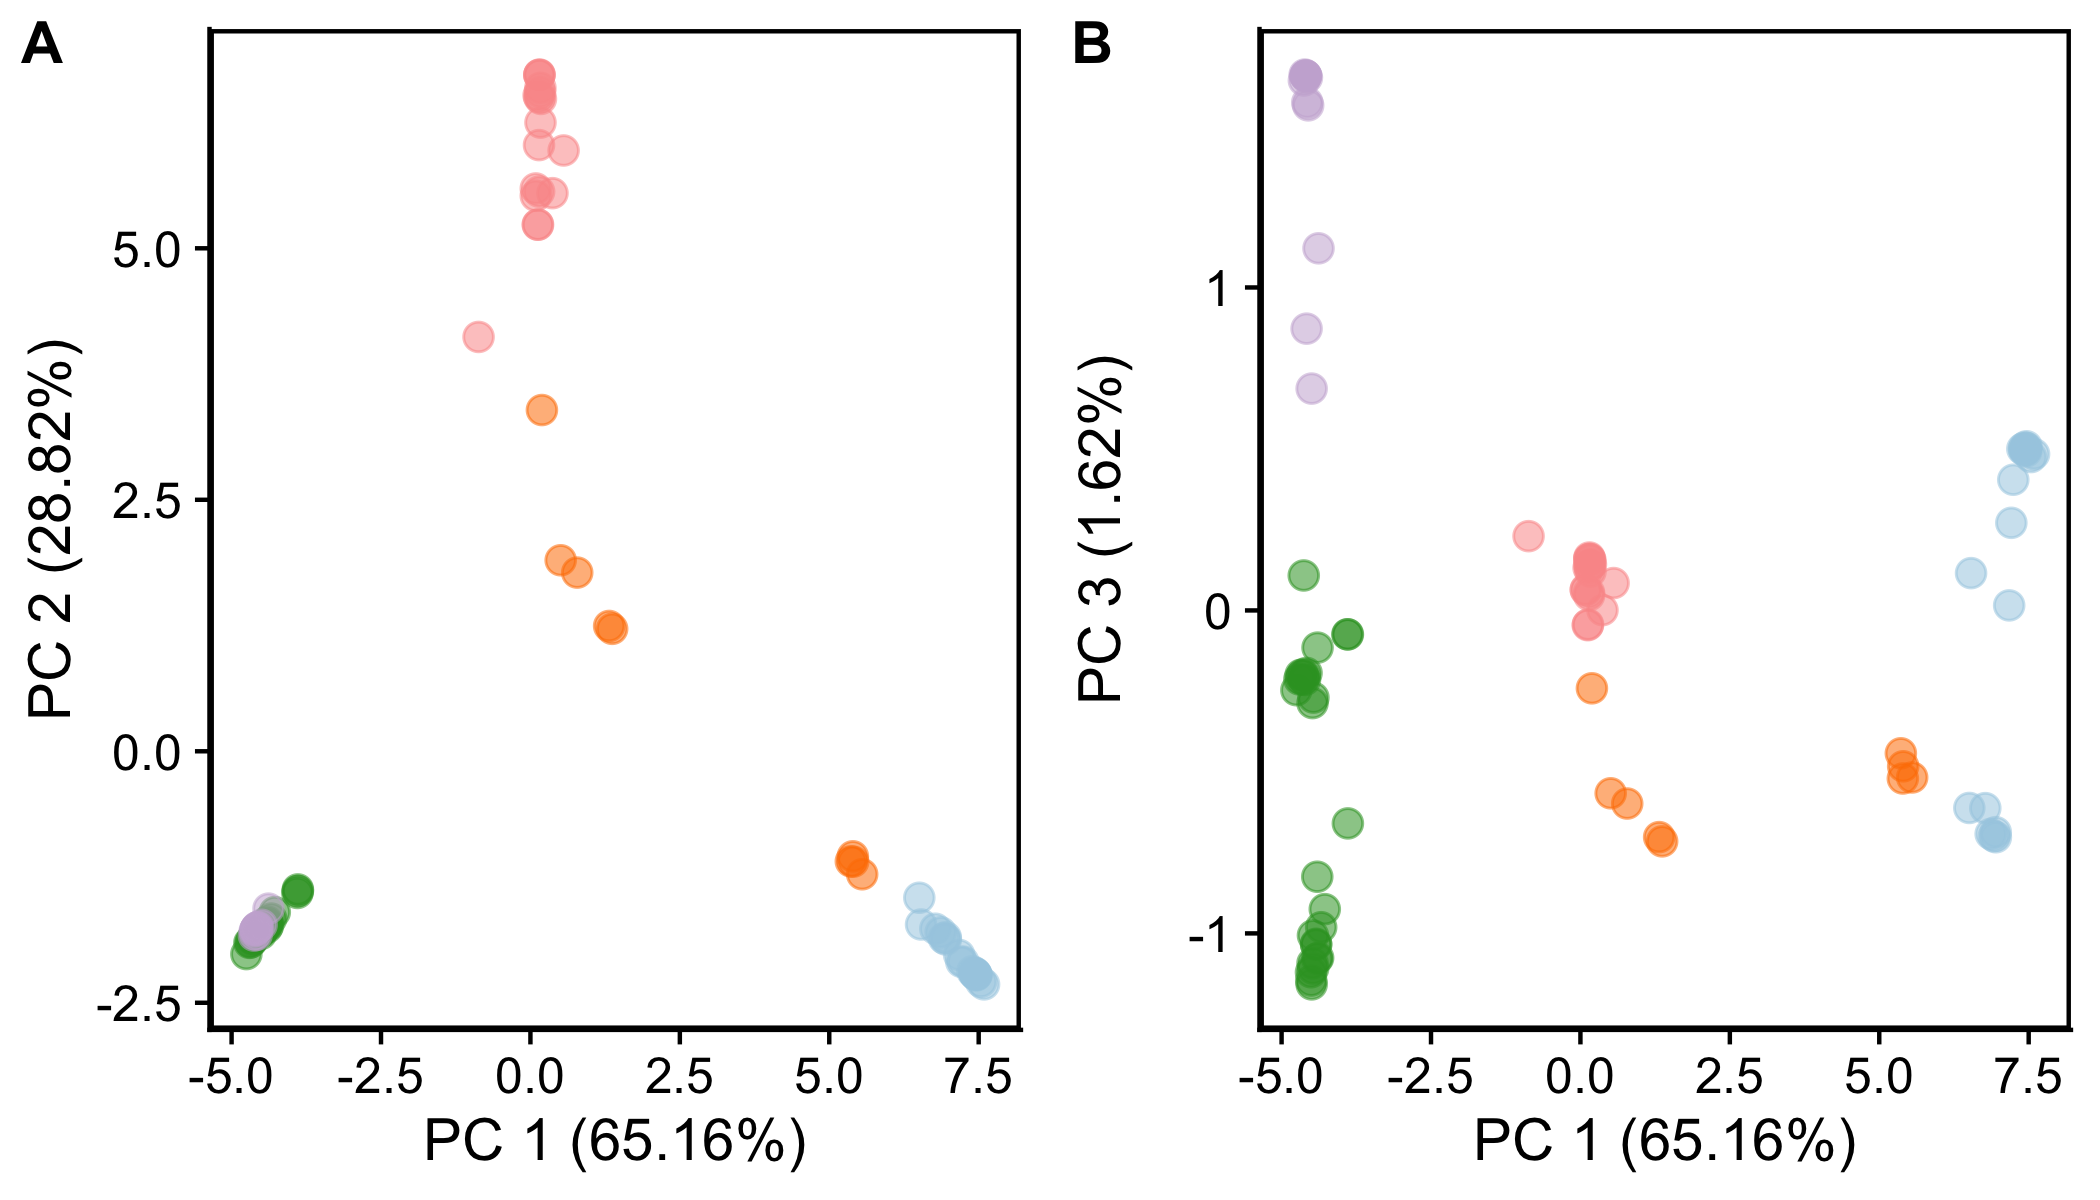
\includegraphics[width=1\linewidth]{figures/pca_plots_side.png}
\caption{\textbf{Principal Component Analysis with filtered samples} Each dot represents each of the 88 samples. \textit{A. caudatus} (green), \textit{A. cruentus} (blue), \textit{A. hybridus} (orange), \textit{A. hypochondriacus} (rose), \textit{A. quitensis} (purple). Axis show the percentage of variance explained by each principal component }
\label{fig:pca}
\end{figure}


\subsection{Categories and Tracks}

We created PopAmaranth relative to the high quality reference genome \citep{lightfoot2017single} and added the gene annotation as functional guide.
We calculated nine summary statistics from the whole genome sequencing data for each of the five species.
The tracks are grouped into five categories, namely annotation, differentiation, diversity, selection and variant calls (Table \ref{tab:tracks}). 
Each category includes tracks one color gradient summary track combining data of a summary statistic for all species.


%\textit{Annotation} Contains the reference tracks, where the reference genome and gene annotation can be found. Chromosomes approximations are represented by the 16 scaffolds, to which add 890 contigs. The nucleotide sequence is visible on the reference genome track. The gene annotation track contains different features; when zoomed out, a barplot is shown representing the gene density for the region. Zooming in makes visible the direction of the gene (represented by an arrow), the exons represented in boxes and the introns om lines. The genes are searchable by their name according to Phytozome annotation. 
 

\subsubsection{Differentiation} 
Tracks in the differentiation category represent all pairwise F$_{st}$ comparisons in 5 kb windows. 
The genome-wide pairwise F$_{st}$ ranged from 0.17 between \textit{A. caudatus} and \textit{A. quitensis} to 0.68 between \textit{A. caudatus} and \textit{A. cruentus}. 
As observed before, F$_{st}$ between crop species was higher than between the crops and their wild ancestor for \textit{A. caudatus} and \textit{A. hypochondriacus} \citep{stetter2020parallel}. 
Although, we found higher F$_{st}$ between \textit{A. cruentus} and \textit{A. hybridus} (0.69) than between \textit{A. cruentus} and \textit{A. hypochondriacus} (0.57).


% | | mean Fst Value |
% |---|---|
% | caudatus/cruentus | 0.681 |
% | cruentus/hypochondriacus | 0.572 |
% | caudatus/hypochondriacus | 0.619 |
% | caudatus/hybridus | 0.325 |
% | caudatus/quitensis | 0.172 |
% | cruentus/hybridus | 0.688 |
% | cruentus/quitensis | 0.730 |
% | hybridus/quitensis | 0.348 |
% | hypochondriacus/hybridus | 0.329 |
% | hypochondriacus/quitensis | 0.676 |




\subsubsection{Diversity} 
The comparison of genetic diversity between different populations can give insights into selection experienced by one population.
Hence, we calculated several diversity statistics along the genome.
Wu \& Watterson $\theta$ and nucleotide diversity ($\pi$) were calculated in 5 kb non-overlapping windows. 
Inbreeding coefficients and expected and observed heterozygosity are reported on a per site basis for each SNP that segregates within a population.
Consistent with previous findings, the three grain amaranths had lower mean $\pi$ (0.005-0.010) compared to their wild ancestor \textit{A. hybridus} (0.019) \citep{stetter2020parallel}. 
Wu \& Watterson $\theta$ was also lower for domesticated amaranth species (0.004-0.007) comparatively to \textit{\textit{A. hybridus} (0.023)}.
In addition, crops had higher average inbreeding coefficients (0.574 in \textit{A. caudatus}, 0.488 in \textit{A. cruentus}, and 0.628 in \textit{A. hypochondriacus} than \textit{A. quitensis} (0.189), but lower than \textit{A. hybridus} (0.676).
 
% # nucleotide diversity (π)
% |  | mean value|
% |---|---|
% | caudatus   |  0.009 |
% |  cruentus |  0.010 |
% |  hypochondriacus |  0.005 |
% | hybridus    |  0.019 |
% | quitensis   |  0.009 |

% #Wu and Watterson estimator (θ)

% |  | mean value|
% |---|---|
% | caudatus   |  0.007 |
% | cruentus |  0.007 |
% | hypochondriacus | 0.005|
% | hybridus    |  0.023|
% | quitensis   |  0.006 |
 
 
% # inbreeding coefficient

% | | mean value|
% |---|---|
% | caudatus | 0.574 |
% | cruentus | 0.488 |
% | hypochondriacus | 0.628 |
% | hybridus | 0.677|
% | quitensis | 0.189 
 
%- domesticated species have :
 % - watterson 0.0062 vs 0.0022 hybridus (0.0058 quitensis)
 % - pi 0.008 (hybridus (0.019) quitensis 0.009
 % - relative pi (hypochondriacus 0.24, caudatus 0.46, cruentus 0.49)
 %- Tajima's D ( 1.19 ) hybridus (-0.59) quitensis (2.03)
% ic caudatus(0.574), cruentus (0.488), hypochondriacus (0.628),hybridus(0.676) quitensis(0.189)


\subsubsection{Selection} 
We calculated three different summary statistics to detect signals of selection along the genome. 
Tracks displaying Tajima's D were calculated in 5 kb windows for each species. 
Tajima's D was higher for domesticated species ( 1.443 in \textit{A. caudatus}, 1.773 in \textit{A. cruentus}, and -0.105 in \textit{A. hypochondriacus} than for their wild ancestor \textit{A. hybridus} (-0.597) indicating a domestication bottleneck. \textit{A. quitensis} had a mean Tajima's D of 2.037 also suggesting a recent population contraction.


% # Tajima's D
% | | mean value|
% |---|---|
% | caudatus | 1.443 |
% | cruentus | 1.773 |
% | hypochondriacus | -0.105 |
% | hybridus | -0.597 |
% | quitensis | 2.037 |
% 

We employed RAiSD to detect signals of selective sweeps in 20 SNP windows within each species. 
The top 1\% of all windows were considered outliers and suggest regions of positive selection.
We found 973 non-overlapping window with signals of positive selection from a total of 1,765,126 windows in \textit{A. caudatus}, 1,096 in 1,654,914 windows in \textit{A. cruentus}, 17,932 in 1,793,173 windows in \textit{A. hypochondriacus}, 2,452 in 4,343,653 windows  in \textit{A. hybridus}, and 1,275 in 1,585,410 windows in \textit{A. quitensis}. 
To investigate the signal of domestication-related selection, we added the relative nucleotide diversity between each crop and their wild ancestor \textit{A. hybridus} in 5 kb windows. 
While the genome-wide $\pi$ was lower for all three crops (see "Diversity"), relative $\pi$ allows to visualize deviations from this genome-wide mean and to detect outlier signals in individual regions.


 %RAisd results
% | species  | total sites detected  | sites>1% threshold  |  nr windows | cut-off |
% |---|---|---|---|---|
% |caudatus | 1765126  |   17650 |  973 | 4.111e-05
% |cruentus   | 1654914  | 16546  | 1096| 5.345e-05   
% |hypochondriacus  | 1793173  |  17932 | 1121 | 5.33828e-05
% |hybridus   | 4343653  |  43415 | 2452 |2.269e-05
% |quitensis   |   1585410 |  15854 | 1275 | 9.241e-05

%% windows average sizes RAisd
% | | average window size|
% |---|---|
% | caudatus | 36055.6 |
% | cruentus | 41195.1 |
% | hypochondriacus | 42156.5 |
% | hybridus | 30257.5 |
% | quitensis | 41940.9 |

\subsubsection{Variant Calls}
For numerous applications it is desirable to select individuals with a certain genetic variant in a region or gene of interest.
Molecular biologists might be interested in evaluating natural alleles of a gene of interest and plant breeders can use individuals with specific variants to enrich their gene pools.
We provide variant data for all five species representing their genotype frequency within the population as pie chart.
Each variant track only displays variants within the given population (not including fixed variants between populations). 
A total of 4,961,210 variants for \textit{A. caudatus}, 4,075,368 for \textit{A. cruentus}, 4,551,278 for \textit{A. hypochondriacus}, 12,238,589 for \textit{A. hybridus}, and 2,342,505 for \textit{A. quitensis} along the genome are available.
 
 
% | species | total sites 
% |---|---|---|
% |caudatus | 4961210 
% |cruentus | 4075368
% |hypochondriacus | 4551278
% |hybridus | 12238589
% |quitensis | 2342505

 
 
% (Figure \ref{fig:Pscreen})
\begin{figure*}[ht]
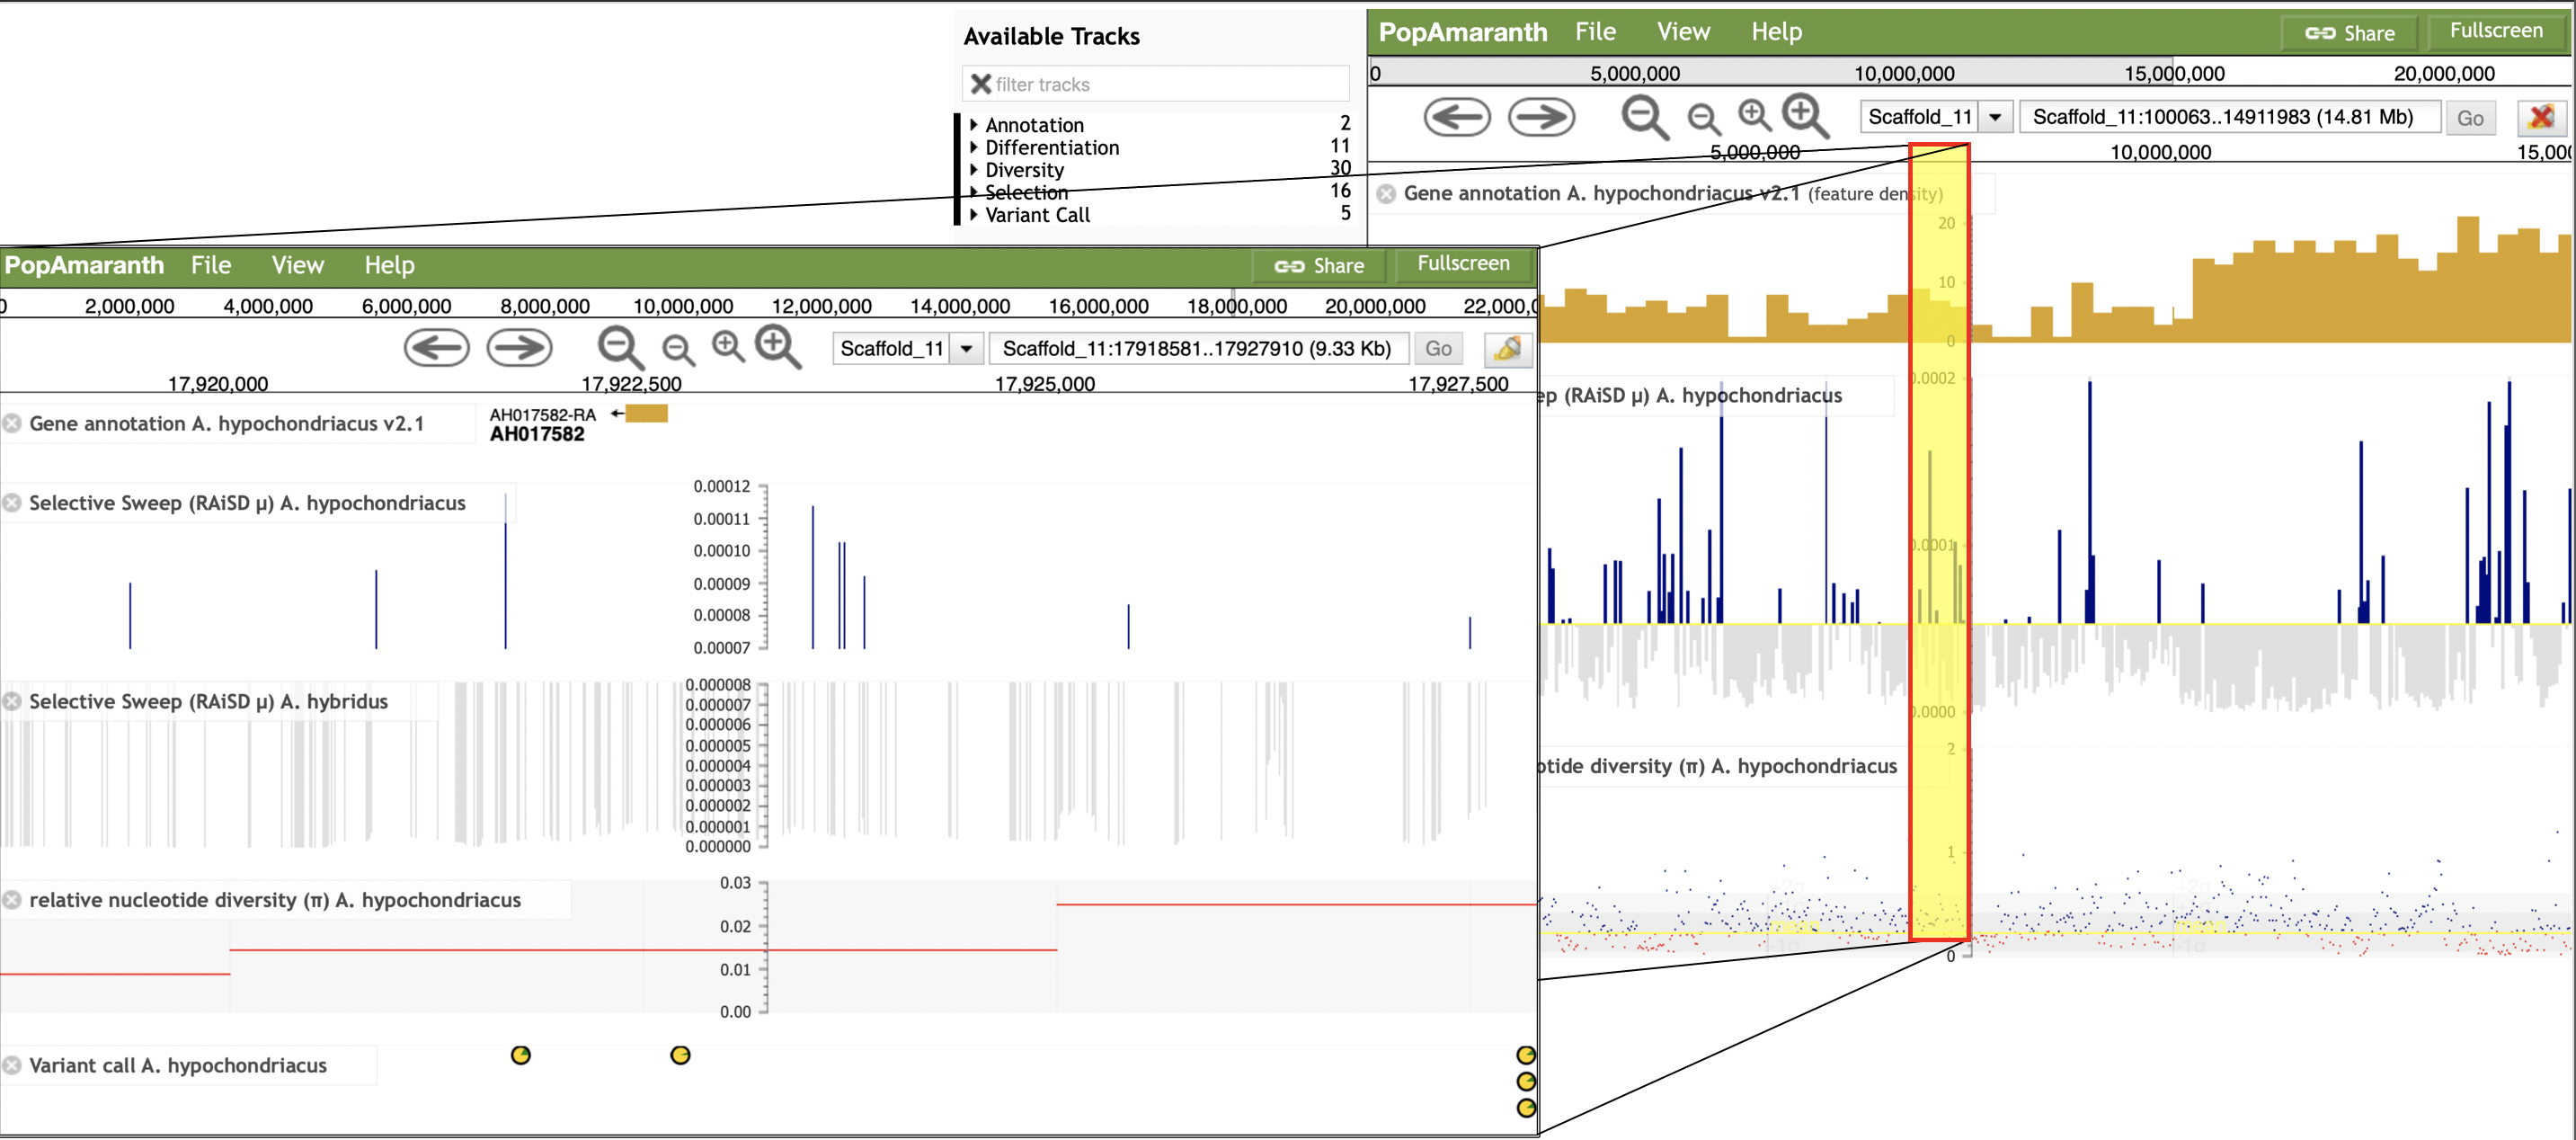
\includegraphics[width=1\linewidth]{figures/figure2_new.png}
\caption{\textbf{PopAmaranth screen view} Background panel: Zoomed out user view along a chromosome. Search field provides access to genome positions or gene names.  Front panel: example is illustrated with a zoom-in region for the water-stress related MIF1 gene (AH-017582).}
\label{fig:Pscreen}
\end{figure*}



 
\begin{table}[htbp]
\centering
\caption{\bf Tracks}
\begin{tableminipage}{0.5\textwidth}
\begin{tabularx}{\textwidth}{sb}
\hline
 Track & Description \\
\hline
\textbf{Annotation} & \\
\hline
Reference Genome v2.0 & \textit{Amaranthus hypochondriacus} reference genome v2.0 \citep{lightfoot2017single} \\
Gene Annotation v2.1 & \textit{Amaranthus hypochondriacus} gene annotation with subfeatures, including CDS, mRNA and UTR's \\
\textbf{Differentiation} & \\
\hline
F$_{st}$ & Fixation Index, average pairwise differences \citet{hudson1992estimation} \\
\textbf{Diversity} & \\
\hline
Wu \& Watterson $\theta$	 & Estimator of Genetic diversity on population \citet{watterson1975number}\\
expected heterozygosity	& Expected rate of heterozygosity for each variant under Hardy-Weinberg equilibrium \\
observed heterozygosity	& Rate of observed heterozygosity for each variant. \\
inbreeding coefficient	& Calculate the inbreeding coefficient for each variant. \\
nucleotide diversity ($\pi$) & Nucleotide diversity \citet{nei1979mathematical}\\
\textbf{Selection} & \\ 
\hline
Tajima's D & difference between the mean number of pairwise differences and the number of segregating sites \cite{tajima1989statistical} \\
relative nucleotide diversity & Ratio of nucleotide diversity between a domesticated species and A. hybridus wild ancestor \\
Selective Sweep (RAiSD ($\mu$) & $\mu$ statistic for selective sweep detection \\
\textbf{Variant Call} & \\
\hline
VCF & called SNP's relative to A. hypochondriacus reference genome\\

\end{tabularx}
 \label{tab:tracks}
\end{tableminipage}
\end{table}
 
% \subsection{Gene MIF1 shows evidence of selection }
\subsection{PopAmaranth case study}
The graphical user interface of PopAmaranth provides a simple way to integrate population genetic and evolutionary results into molecular studies. 
To show the utility of our tools, we evaluated the evolutionary signals within genes that were molecularly shown to be involved in the response of \textit{A. hypochondriacus} to water stress \citep{huerta2011water}. 
We found that MIF1 (AH-017582) showed lower nucleotide diversity, decreased expected heterozygozity, and relative nucleotide diversity below the genome-wide average in all three grain amaranth species. 
In addition, we identified a selective sweep signature in \textit{A. hypochondriacus} around this gene (Figure \ref{fig:Pscreen}). 

In addition to the amaranth specific use, PopAmaranth facilitates the evaluation of hypothesis beyond the species.
To show its utility to study convergent selection signals across distant families, we evaluated population genetic signals around the amaranth ortholog to the triterpene saponin biosynthesis activating regulator 1 - TSAR1 (AH-019562), a key regulator for seed saponin content in \textit{Chenopodium quinoa} \citep{jarvis2017genome}.
We found signals of selective sweeps on the three grain amaranth species. 
%Furthermore, the relative nucleotide diversity was below the genome-wide mean in all grain amaranths within the region around AmTSAR1, suggesting selection during amaranth domestication.
Furthermore, the relative diversity compared to the wild ancestor was below the genome-wide mean, suggesting selection during amaranth domestication (Figure \ref{fig:sponin_sup}).

The above examples show the utility of PopAmaranth for the amaranth community and beyond. 
In addition to the user-friendly evaluation of evolutionary signals in multiple amaranth species, the browser can be used to identify distinct genotypes with diverging alleles in genes of interest to study the molecular function of these genes in amaranth.
%Saponins confer toxicity that, for instance,can protect the crop against attack by birds \citep{rastrelli1995studies, rastrelli1998studies, oleszek1999determination, mroczek2015phytochemistry}. 
%Saponins are widely present on plants and therefore PopAmaranth can provide insights in interspecies studies, aiding in the identification of convergent evolutionary traits.


%- low nucleotide diversity (except hybridus)
%- low watterson (except hybridus)
%- relative pi inferior (redundant ??)
%- Tajima higher
%- Selective Sweeps found aroud it
%- Low heterozygosity on the region

%\subsection{Gene MYBL-1 (AH-014566) }
%- Targeted showed signs of selection
 %- low Tajima D hypochondriacus hybridus
 %- relative pi specially low in caudatus, but below in all three domesticated species
%- MYB candidate has signals of selection upstream of the gene. This might indicate that the regulation of gene color is an adaptive trait (or consequence of domestication (elaborate)) 
%- no selective sweeps
%- observed heterozygosity below mean in all except hybridus
%- inbreeding coefficient above mean in all species

 

%%%%%%%%%%%%%%%%%%%%%%%%%%%%%%%%%%%%%%%%%%%%%%%%%%%%%%%%%%%%%%%%%%%%%


\section{Discussion}

Over the last decades, large-scale population genomic data revealed insights into the evolution and adaptation of crops.
Providing access to results in a user-friendly and interactive way opens paths to better integrate data from different research areas.
Our population genomic genome browser, PopAmaranth, aims to provide such an intuitive tool for amaranth population genetic results.
The inclusion of five different species involved in the domestication history of the crop facilitates hypothesis testing along this evolutionary gradient.

A sampling of distinct populations is crucial for a reference tool as miss-classified samples would confound population-wide signals \citep{rieseberg2004plant, gutierrez2018genetic}. %meier2019tygs
Therefore, we only selected unambiguous samples of each species, base on morphological and genetic classifications.
Our sub-sampling approach is conservative regarding genetic diversity, as it excludes more differentiated individuals from the analysis. 
Regarding genetic differentiation (F$_{st}$) between species, the sub-sampling could lead to an overestimation due to the lack of intermediate individuals. 
The increased differentiation by sub-sampling potentially led to the higher F$_{st}$ value between \textit{A. cruentus} and \textit{A. hybridus} compared to previous results \citep{stetter2020parallel}.
While there is a trade-off between including additional individuals and the potential for undiscovered diversity, our goal was a defined and distinguished set of samples representing each species.
The inclusion of only core individuals of each species further allows the comparison and classification of less distinct individuals using our set.
%The unified estimation of numerous population genetic parameters with a clearly defined set of individuals and similar filtering provides a step towards building an amaranth genomics community. 

For other plant species, i.e., maize \citep{lawrence2004maizegdb}, tomato \citep{fernandez2015sol}, and arabidopsis \citep{weigel20091001, 1001:2016}, accessible platforms of genomic and evolutionary data are integral parts of the research communities. 
We hope that PopAmaranth and the higher level framework amaranthGDB will help establish an amaranth community that benefits from the interdisciplinary exchange.
The browser framework allows the addition of more tracks of evolutionary importance, i.e., levels of introgression between species and genotype-phenotype correlations as generation through genome-wide association mapping.

%PopAmaranth represents a user-friendly tool to evaluate population genetic signals of candidate genes. 
Our results show how PopAmaranth can be employed to add an evolutionary perspective to different molecular questions. 
We identify previously unknown signals of selection in stress-related MIF1 gene, which might have been under selection during amaranth domestication. 
In most crops, domestication led to a reduction in stress resilience compared to their wild ancestors. 
Hence the reduction in diversity might represent selection against the tolerant allele to free resources for increased crop productivity \citep{koziol2012reduced}. 
Our browser allows the selection of genotypes with different alleles within grain amaranths and in wild amaranth, which can lead to the identification of stress-tolerance alleles and potentially the reintroduction of such alleles into breeding programs.

On a broader scale, PopAmaranth also facilitates the comparison of convergent adaptation signals between more distant taxa. 
For instance, our finding of convergent selection between quinoa and amaranth in a saponin-related gene suggests that in both quinoa and amaranth the saponin content was reduced to improve the palatability of the grains \citep{jarvis2017genome}. 
Saponins confer toxicity protect wild plants against bird but reduce the nutritional quality of seeds for human consumption and animal feed \citep{rastrelli1995studies, rastrelli1998studies, oleszek1999determination, mroczek2015phytochemistry}. 
Hence, our platform allowed to identify the convergent selection between the two pseudocereals, demonstrating its utility to evaluate selection signals across taxa.

\section{Conclusion}

We present and employ PopAmaranth, a population genetic genome browser that provides an interactive way to identify evolutionary signals along the amaranth genome.
We incorporated a well-defined set of individuals with congruent data filtering to estimate population-wide diversity statistics for the three grain amaranth species and two wild relatives. 
The identification of selection signals in candidate genes within amaranth and beyond shows the utility of the browser for a range of researchers.
PopAmaranth and the amaranthGDB platform will help to build and grow the amaranth research community and facilitate interdisciplinary research to ultimately improve the crop.

\section{Availability}

JBrowse is available at \url{https://amaranthgdb.org/popamaranth/}.



\section{Acknowledgments}
We thank the RRZ team at University of Cologne, for hosting PopAmaranth, the de Meaux lab for testing and feedback on the browser, and all the Stetter Lab for discussion. 

 

\bibliography{bib}

%\pagebreak
\onecolumn
\section*{Supplement}


 
\beginsupplement

\begin{figure*}[ht]
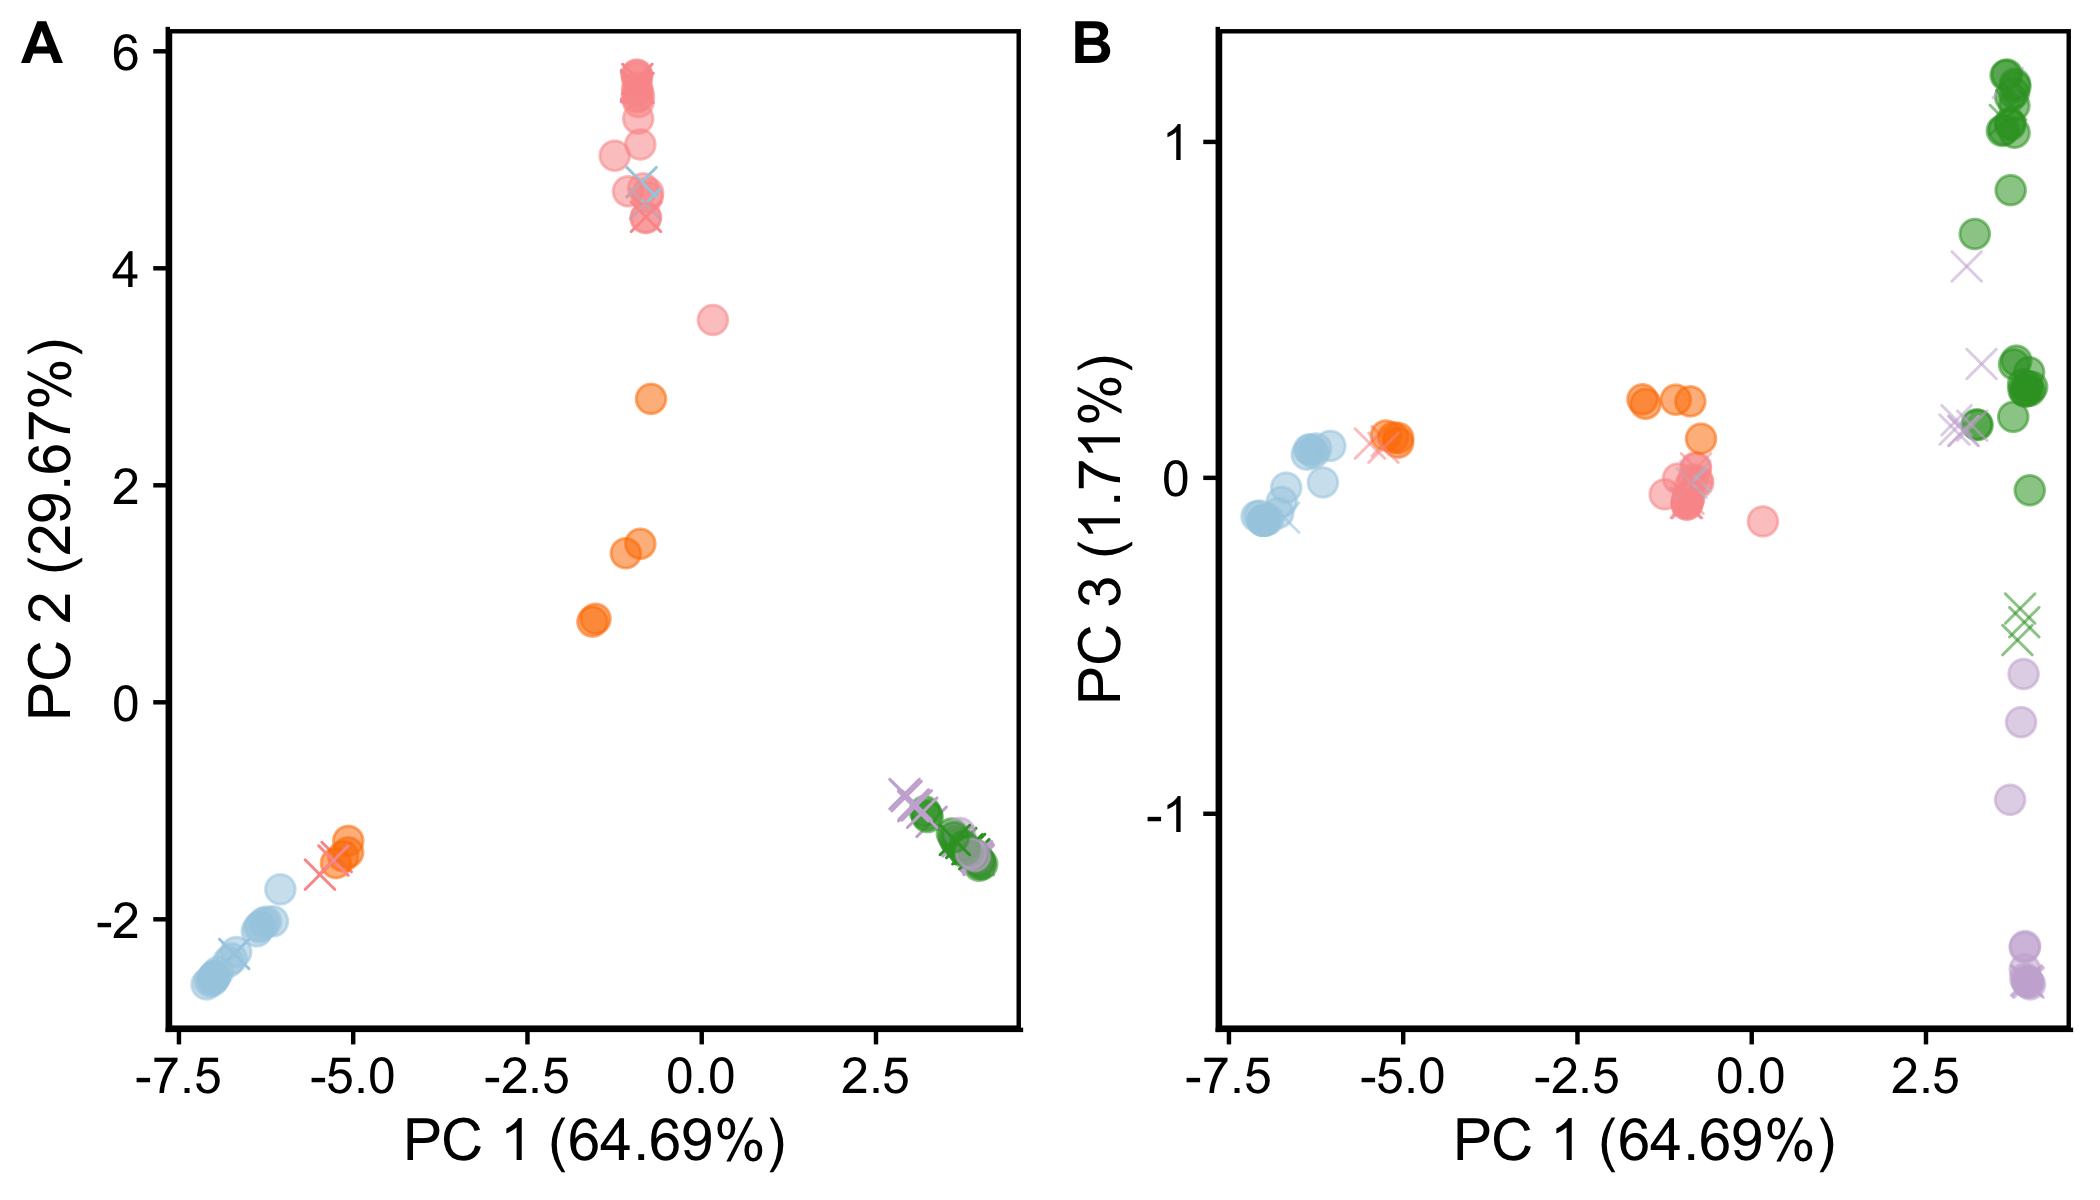
\includegraphics[width=1\linewidth]{figures/pca_plots_all_samples.png}
\caption{\textbf{PCA before filtering.} Each symbol represents each of the 116 sample. Circles represent amaranth samples included in the study. Removed samples are marked with crosses. \textit{A. caudatus} (green), \textit{A. cruentus} (blue), \textit{A. hybridus} (orange), \textit{A. hypochondriacus} (rose), \textit{A. quitensis} (purple). Axis show the percentage of variance explained by each principal component.}
\label{fig:pca_sup}
\end{figure*}




\begin{figure*}[ht]
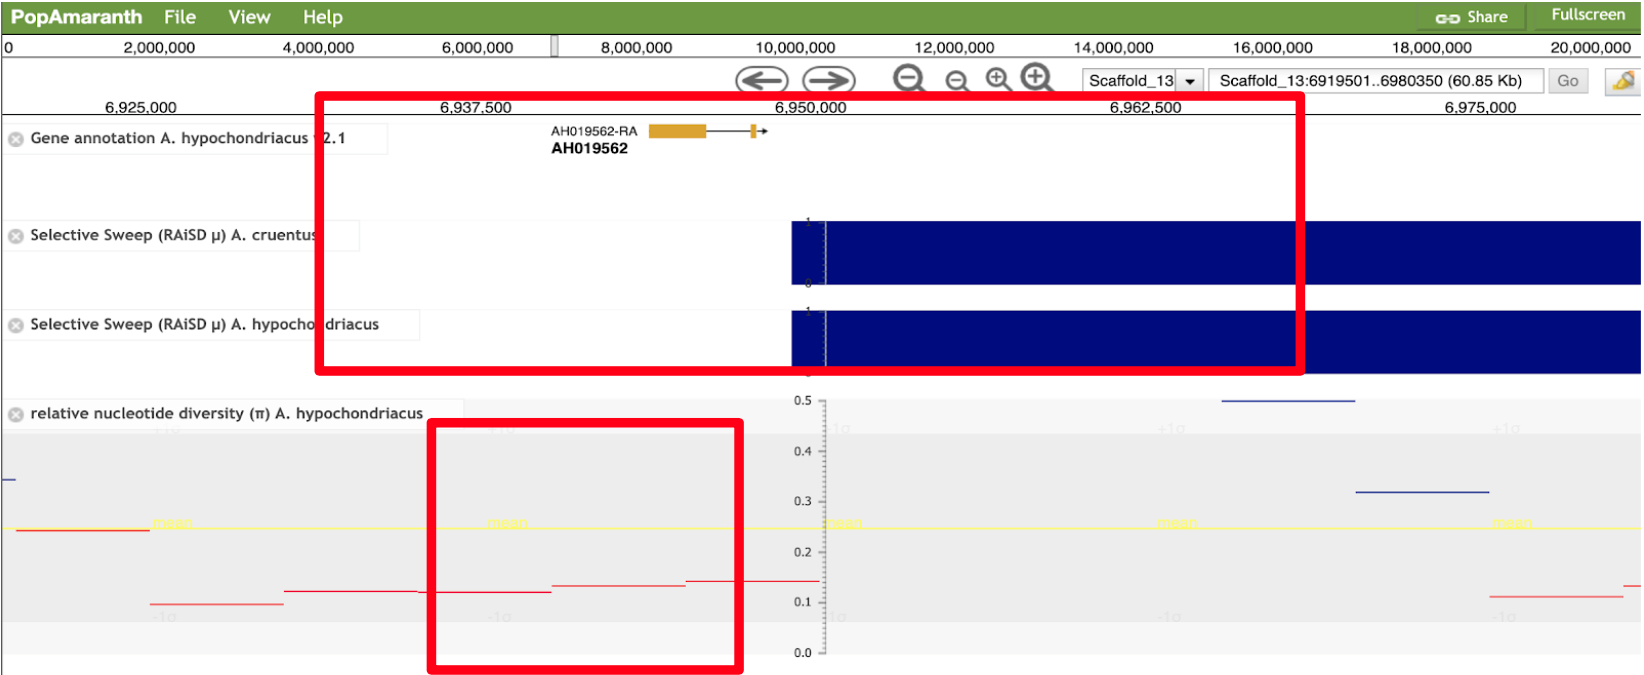
\includegraphics[width=1\linewidth]{figures/Saponin_region_highlight.png}
\caption{\textbf{AmTSAR1 (AH-019582)}.  Sceenshot of the gene region. Signals of positive selection identified in \textit{A. cruentus} and \textit{A. hypochondriacus}. Relative nucleotide diversity between A. hypochindriacus compared to its wild ancestor \textit{A. hybridus} is lower than the genome wide relative diversity, indicating selection in this region.}
\label{fig:sponin_sup}
\end{figure*}



\pagebreak
\small
\begin{longtable}{p{3cm}p{6cm}p{8cm}}

\caption{Detailed description of the included categories (bold) and respective tracks and summary statistics}\\
\hline
\textbf{ Track Name} & \textbf{Description} & \textbf{Detailed explanation} \\\hline
\endfirsthead
\multicolumn{3}{c}%
{\tablename\ \thetable\ -- \textit{Continued from previous page}} \\
\hline
\textbf{ Track Name} & \textbf{Description} & \textbf{Detailed explanation} \\
\hline
\endhead
\hline \multicolumn{3}{r}{\textit{Continued on next page}} \\
\endfoot
\hline
\endlastfoot
\hline
\textbf{Annotation} & & \\
\hline
Reference Genome v2.0 & \textit{Amaranthus hypochondriacus} reference genome v2.0 \citep{lightfoot2017single} & Reference sequence of the A. hypochondriacus (version 2.0 from Phytozome) \citep{goodstein2012phytozome} \\
Gene Annotation v2.1 & \textit{Amaranthus hypochondriacus} gene annotation with subfeatures. & Follows Phytozome nomenclature for gene names. Clicking on the track, information for subfeatures CDS, mRNA, and UTR’s is present. For each of the subfeatures, its name, type, position on the chromosome, and length are described. \textit{Gene density} viewable from whole chromosome perspective. \\
\textbf{Differentiation} & & \\ 
\hline
F$_{st}$ & Weir-Cockerham pairwise F$_{st}$ \citet{weir1984estimating} & pairwise F$_{st}$ between species pairs calculated on non-overlapping 5 kb windows. Windows with F$_{st}$ below the mean are represented in red and above the mean in blue. Shading in light and darker grey represents 1$\sigma$ and 2$\sigma$ from the mean, respectively. A red window indicates a region with higher fixation of alleles (genetic differentiation) between the two species, and the opposite for a blue window. The yellow line represent the global mean F$_{st}$. %If two populations have a F$_{st}$ of 1, it means the populations are fixed for different alleles. 
For visualization purposes, scale is adjusted for the local values of the region in display.\\
& & 	\textit{Summary F$_{st}$}: Color gradient showing F$_{st}$ values for all comparisons in a compact way. Color scale varies from white (0) to darker blue (1). Each bar represents the value of one 5kb window. \\
\textbf{Diversity} & & \\
\hline
Wu \& Watterson $\theta$ & Estimator of Genetic diversity on population \citet{watterson1975number}& $\theta$ for each pairs calculated on non-overlapping 5 kb windows. Windows with $\theta$ below the mean are represented in red and above the mean in blue. Shading in light and darker grey represents 1$\sigma$ and 2$\sigma$ from the mean, respectively. The yellow line represent the global mean $\theta$. The lower the $\theta$, the lower the genetic diversity within the population. For visualization purposes, scale is adjusted for the local values of the region in display. \\
& & 	\textit{Summary Wu \& Watterson $\theta$}: Color gradient showing $\theta$ values for all comparisons in a compact way. Color scale varies from white (0) to darker blue (1) . Each bar represents the value of one 5kb window.\\
expected heterozygosity	& Expected rate of heterozygosity for each variant under Hardy-Weinberg equilibrium & SNP-based expected heterozygosity are represented in blue when above the mean and in red when expected heterozygosity is below the mean. The yellow line represent the global mean expected heterozygosity. Values range between 0 and 1. For visualization purposes, scale is adjusted for the local values of the region in display. \\
& & 	\textit{Summary expected heterozygosity}: Color gradient showing expected heterozygosity values for all comparisons in a compact way. Color scale varies from white (0) to darker blue (1) . Each bar represents the value for each variant.\\
observed heterozygosity	& Rate of observed heterozygosity for each variant. & SNP- based observed heterozygosity are represented in blue when above the mean and in red when observed heterozygosity is below the mean. The yellow line represent the global mean observed heterozygosity. Values range between 0 and 1. For visualization purposes, scale is adjusted for the local values of the region in display .
Each bar represents the value for each variant.\\
& & 	\textit{Summary observed heterozygosity}: Color gradient showing observed heterozygosity values for all comparisons in a compact way. Color scale varies from white (0) to darker blue (1) . Each bar represents the value for each variant.\\
inbreeding coefficient	& Calculation of the inbreeding coefficient for each variant. & Calculated based on observed heterozygosity and expected heterozygosity.
SNP-based inbreeding coefficient are represented in blue when above the mean and in red when the inbreeding coefficients below the mean. The yellow line represent the global mean inbreeding coefficient. Values range between 0 and 1. For visualization purposes, scale is adjusted for the local values of the region in display.\\
& & 	\textit{Summary inbreeding coefficient}: Color gradient showing inbreeding coefficient values for all comparisons in a compact way. Color scale varies from white (0) to darker blue (1) . Each bar represents the value for each variant.\\
nucleotide diversity ($\pi$) & Nucleotide diversity \citet{nei1979mathematical} & Windows of 5kb with average number of nucleotide differences above the mean are represented in blue and are represented in red when $\pi$ is below the mean. The yellow line represent the global mean $\pi$. Shading in light and darker grey represents 1$\sigma$ and 2$\sigma$ from the mean, respectively. For visualization purposes, scale is adjusted for the local values of the region in display. A track is available for each species.\\
& & 	\textit{Summary nucleotide diversity ($\pi$}: Color gradient showing $\pi$ values for all comparisons in a compact way. Color scale varies from white (0) to darker blue (1) . Each bar represents the value for each variant.\\

\textbf{Selection} & & \\ 
\hline 
Tajima's D & difference between the mean number of pairwise differences and the number of segregating sites \cite{tajima1989statistical} & Deviations from neutral state (Tajima's D=0) are possible signals of selection or demographic changes. 
%Tajima’s D <0, describes an excess or rare alleles from a selective sweep or population expansion after a recent bottleneck occurred. Tajima’s D > 0 describes a lack of rare alleles and indicates balancing selection or a sudden population contraction. Tajima’s D = 0 means that the population is under mutation-drift equilibrium. 
Windows of 5kb with Tajima's D above the mean are represented in blue and in red when the values are below the mean . A track is available per species. Shading in light and darker grey represents 1$\sigma$ and 2$\sigma$ from the mean, respectively. The yellow line represent the global mean Tajima's D. For visualization purposes, scale is adjusted for the local values of the region in display.\\
& & 	\textit{Summary Tajima's D}: Color gradient showing Tajima's D values for all comparisons in a compact way. Color scale varies from red (<0) to white (0) to darker blue (1). Each bar represents the value of one 5kb window. \\
relative nucleotide diversity & Ratio of nucleotide diversity between a domesticated species and A. hybridus wild ancestor & Ratio between the nucleotide diversity of two amaranth species. Tracks are available for each of the grain amaranth species (\textit{A. caudatus}, \textit{A. cruentus}, \textit{A. hypochondriacus}) relative to the wild ancestor (A. hybridus). Windows of 5kb above the mean are represented in blue and windows below the mean are represented in red. For visualization purposes, scale is adjusted for the local values of the region in display. \\ 
 
Selective Sweep (RAiSD ($\mu$) & $\mu$ statistic for selective sweep detection & Each bar represents the window center of a 20 SNP region with the top 1\% $\mu$ values copared to all 20 SNP windows. These outliers indicate regions with signals of positive selection and are displayed as blue bars.\\
& & 	\textit{Summary Selective Sweep (RAiSD ($\mu$)}: Color gradient showing $\mu$ values for all comparisons in a compact way. Blue colored regions represent regions with putative signals of positive selection.\\
\textbf{Variant Call} & &\\
\hline
VCF & Single nucleotide polymorphisms (SNP) identified.& Variant calls from \citet{stetter2020parallel} within each amaranth species. Genotypes are displayed in pie charts. Gold colored slices represent the percentage of homozygous reference genotypes, green all other genotypes (heterozygous and homozygous alternative).\\ 

\end{longtable}
% \end{center}
\end{document}

 



Anonymous Usage Statistics in order to
follow ‘SCCs’ [Standard Contractual Clauses], GDPR?? we opt out to provide JBrowse instances report usage statistics to the JBrowse developers . suppressed usage statistics 

\pagebreak


\end{document}
